\documentclass[a4paper]{article}
\usepackage[francais]{babel}
\usepackage[utf8x]{inputenc}
\usepackage[T1]{fontenc}
\usepackage[a4paper,top=3cm,bottom=2cm,left=3cm,right=3cm,marginparwidth=1.75cm]{geometry}
\usepackage{amsmath}
\usepackage{graphicx}
\usepackage[colorinlistoftodos]{todonotes}
\usepackage{amssymb}
\usepackage[colorlinks=true, allcolors=blue]{hyperref}

\title{INFO-F-302 Informatique Fondamentale \\ Rapport du projet 2016-2017}
\author{Nathan~Liccardo, Stanislas~Gueniffey}

\begin{document}
\maketitle

\section{Introduction}
La projet détaillé dans ce document avait deux objectifs : la modélisation de problèmes sous formes CSP et l'implémentation de ceux-ci en Java. Les réponses fournies seront formalisées selon le modèle CSP à savoir : variables, domaines et contraintes.

\section{Problèmes d'échecs}
Nous supposons ici que le lecteur est familier avec le \href{https://fr.wikipedia.org/wiki/%C3%89checs}{jeu d'échecs}. Les problèmes posés par la suite consistent à reproduire des scénarios plausibles dans le cadre d'une partie de ce jeu, dont certains paramètres ont été modifiés et respectant des contraintes supplémentaires (qui elles ne sont pas inhérentes au jeu).

\subsection{Formalismes}
Afin de pouvoir obtenir le problème sous la forme d'un CSP, nous avons posé certaines variables inhérentes au problème : 
\begin{center}
\begin{tabular}{|c|c|}
\hline
n & La taille du tableau d'échecs \\
\hline
$k_1$ & Le nombre de tours \\
\hline
$k_2$ & Le nombre de fous \\
\hline
$k_3$ & Le nombre de cavaliers  \\
\hline
\end{tabular}
\end{center}

\subsection{Problème d'indépendance}
Le problème d’indépendance consiste à déterminer s’il est possible d’assigner à chacune des pièce une position distincte sur l'échiquier de sorte qu’aucune pièce ne menace une autre pièce.\\ 
\begin{center}
\fbox{\fbox{\parbox{5.5in}{\centering
Exprimer une instance quelconque du problème d'indépendance par un CSP équivalent, en exposant de manière claire les variables, leurs domaines respectifs et les contraintes à respecter. 
}}}
\end{center}

\subsubsection{Variables}
Nous avons défini dans un premier temps les variables représentant respectivement les tours, les fous et les cavaliers : 
\begin{center}
$X = \{ x_t | \ t \in K1 \}  \cup \{ x_f | \ f \in K2 \} \cup \{ x_c | \ c \in K3 \}$
\end{center}
Par facilité de notation, nous avons également définit les ensembles suivants qui sont directement liés aux places et pièces du jeu : 
\begin{equation*}
N = \{1,\ldots,n\}
\end{equation*}
\begin{equation*}
K_1 = \{ t_1,\ldots,t_{k1} \}
\end{equation*}
\begin{equation*}
K_2 = \{ f_1,\ldots,f_{k2} \}
\end{equation*}
\begin{equation*}
K_3 = \{ c_1,\ldots,c_{k3} \}
\end{equation*}
\begin{equation*}
K = K_1 \cup K_2 \cup K_3
\end{equation*}
\begin{equation*}
K_4 = \{ v_1,\ldots,v_{(n*n)-(k_1+k_2+k_3)} \}
\end{equation*}
\subsubsection{Domaines}
Les pièces seront représentées sous la forme de coordonnées $X$ et $Y$. Ce sont ces deux valeurs qui formeront le domaine pour les trois types de pièces : 
\begin{center}
$D_t = \{ (i,j) | 1 \leq i \leq n \wedge 1 \leq j \leq n \}$ \\
$D_f = \{ (i,j) | 1 \leq i \leq n \wedge 1 \leq j \leq n \}$ \\
$D_c = \{ (i,j) | 1 \leq i \leq n \wedge 1 \leq j \leq n \}$
\end{center}
\subsubsection{Contraintes}
Les contraintes s'appliquants sur les variables de ce problème doivent prendre en compte les deux demandes suivantes : 
\begin{center}
\textit{Une case est occupée par maximum une pièce.} \vspace{0.1cm} \\
\textit{Aucune pièce ne peut en menacer une autre.} 
\end{center}
Notre ensemble de contraintes final sera l'union entre les contraintes de positions et les contraintes de domination : 
\begin{equation*}
C = C_p \cap C_d
\end{equation*}
Définissons dans un premier temps l'ensemble correspondant aux contraintes de positions. Ce dernier reprendra alors l'ensemble des contraintes liants les différentes pièces entre-elles : 
\begin{equation*}
C_p = \{ C_{p_lp_m} | \  p_l \in K, p_m \in K \backslash \{ p_l \} \}
\end{equation*}
Voici le détail de la contrainte : 
\begin{equation*}
C_{p_lp_m} = ((x_{p_l},x_{p_m}), \{ (i_{p_l},j_{p_m},i_{p_l},j_{p_m}) \in N^4 \ | \ \neg((i_{p_l} = i_{p_m}) \wedge (j_{p_l} = j_{p_m})) \})
\end{equation*}
Nous allons à présent définir l'ensemble correspondant aux contraintes de dominations. Ce dernier permettra de s'assurer qu'aucune pièce n'en menace une autre : 
\begin{align*}
\begin{split}
C_d ={}& \{ C_{t_lp_m} | \ t_l \in K_1, p_m \in K \backslash \{ t_l \} \} \ \cap \\
	    & \{ C_{f_lp_m} | \ f_l \in K_2, p_m \in K \backslash \{ f_l \} \} \ \cap \\
	    & \{ C_{c_lp_m} | \ c_l \in K_3, p_m \in K \backslash \{ c_l \} \}
\end{split}
\end{align*}
Voici à présent le détail des diverses contraintes :  
\begin{align*}
\begin{split}
C_{t_lp_m} = ( (x_{t_l},x_{p_m}), \{ (i_{t_l},i_{p_m},j_{t_l},j_{p_m}) \in N^4 | & \neg( [ (i_{t_l} = i_{p_m}) \vee(j_{t_l} = j_{p_m}) ]\wedge \\
& [(i_{t_l} = i_{p_m}) \rightarrow (\nexists \ x_p, \{ p \in K \backslash \{t_l,p_m\} | i_{p} = i_{t_l} \wedge j_p \in \{ j_{t_l},...,j_{p_m} \}] \wedge \\
&[(j_{t_l} = j_{p_m}) \rightarrow (\nexists \ x_p, \{ p \in K \backslash \{t_l,p_m\} | j_p = i_{t_l} \wedge i_p \in \{ i_{t_l},...,i_{p_m} \}\}  ] ) \} )
\end{split}
\end{align*}

\begin{align*}
\begin{split}
C_{f_lp_m} = ( (x_{f_l},x_{p_m}), \{ (i_{f_l},i_{p_m},j_{f_l},j_{p_m}) \in N^4 | & \neg( [ abs(i_{f_l} - i_{p_m}) = (abs(j_{f_l} - j_{p_m})) ]\wedge \\
& [ \nexists \ x_p, \{ p \in K \backslash \{f_l,p_m\} | i_{p} \in \{ i_{t_l},...,i_{p_m} \} \wedge j_p \in \{ j_{t_l},...,j_{p_m} \}\}  ] ) \} )
\end{split}
\end{align*}

\begin{align*}
\begin{split}
C_{c_lp_m} = ( (x_{c_l},x_{p_m}), \{ (i_{c_l},i_{p_m},j_{c_l},j_{p_m}) \in N^4 |& (abs(i_{c_l} - i_{p_m}) \neq 2 \wedge abs(i_{c_l} - i_{p_m}) \neq 1) \wedge \\
& (abs(i_{c_l} - i_{p_m}) \neq 1 \wedge abs(i_{c_l} - i_{p_m}) \neq 2)\} \} )
\end{split}
\end{align*}
Nous pouvons maintenant affirmer que le respect de ces contraintes sur les variables fournies nous permettra d'obtenir le résultat du problème d'indépendance. 

\subsection{Problème de domination}
Le problème de domination consiste à déterminer s’il est possible d’assigner à chacune des pièce une position distincte sur l'échiquier de sorte que chaque case soit occupée ou menacée par au moins une pièce.

\begin{center}
\fbox{\fbox{\parbox{5.5in}{\centering
Exprimer une instance quelconque du problème de domination par un CSP équivalent, en exposant de manière claire les variables, leurs domaines respectifs, et les contraintes à respecter.
}}}
\end{center}

\subsubsection{Variables}
Les variables seront définies de la même manière que pour l'exercice précédent. Nous créons cependant une nouvelle variable représentant les cases vides : 
\begin{center}
$X = \{ x_t | \ t \in K1 \}  \cup \{ x_f | \ f \in K2 \} \cup \{ x_c | \ c \in K3 \} \cup \{ x_v | \ v \in K4 \}$
\end{center}
Par facilité de notation, nous avons également définit les ensembles suivants qui sont directement liés aux places et pièces du jeu : 
\begin{equation*}
N = \{1,\ldots,n\}
\end{equation*}
\begin{equation*}
K_1 = \{ t_1,\ldots,t_{k1} \}
\end{equation*}
\begin{equation*}
K_2 = \{ f_1,\ldots,f_{k2} \}
\end{equation*}
\begin{equation*}
K_3 = \{ c_1,\ldots,c_{k3} \}
\end{equation*}
\begin{equation*}
K = K_1 \cup K_2 \cup K_3
\end{equation*}
\begin{equation*}
K_4 = \{ v_1,\ldots,v_{(n*n)-(k_1+k_2+k_3)} \}
\end{equation*}

\subsubsection{Domaines}
Les domaines sont définis de façon identique au problème précédent pour l'ensemble des pièces mises à disposition : 
\begin{center}
$D_t = \{ (i,j) \ | \ 1 \leq i \leq n \wedge 1 \leq j \leq n \}$ \\
$D_f = \{ (i,j) \ | \ 1 \leq i \leq n \wedge 1 \leq j \leq n \}$ \\
$D_c = \{ (i,j) \ | \ 1 \leq i \leq n \wedge 1 \leq j \leq n \}$ \\
\end{center}
Etant donné la présence de nouvelles variables, il faut également ajouté le domaine s'y appliquant à savoir : 
\begin{center}
$D_v = \{ (i,j) \ | \ 1 \leq i \leq n \wedge 1 \leq j \leq n \}$
\end{center}

\subsubsection{Contraintes}
Les contraintes appliquées dans le cas du problème de domination seront quant à elles légèrement différentes. Dans ce nouveau problème, nous avons l'affirmation suivante qui doit être respectée :
\begin{center}
\textit{L'ensemble des cases libres doivent être menacées.} \vspace{0.1cm} \\
\textit{Une case est occupée par maximum une pièce.}
\end{center}
Dans ce second problème, notre ensemble de contrainte sera alors composé des contraintes de menaces et des contraintes de positions : 
\begin{align*}
C = C_m \cap C_p
\end{align*}
Nous allons commencer par définir l'ensemble de contraintes $C_p$. Cet ensemble représentera l'impossibilité de positionner deux pièces sur la même case : 
\begin{equation*}
C_p = \{ C_{p_lp_m} | \  p_l \in K, p_m \in K \backslash \{ p_l \} \}
\end{equation*}
Il sera alors défini de la façon suivante : 
\begin{equation*}
C_{p_lp_m} = ((x_{p_l},x_{p_m}), \{ (i_{p_l},j_{p_m},i_{p_l},j_{p_m}) \in N^4 \ | \ \neg((i_{p_l} = i_{p_m}) \wedge (j_{p_l} = j_{p_m})) \})
\end{equation*}
Nous pouvons à présent détailler l'ensemble permettant d'appliquer les menaces sur chaque cases vides : 
\begin{align*}
\begin{split}
C_m ={} & \{ C_{v_lt_m} | \ v_l \in K_4, t_m \in K_1 \} \ \cup \\
	      & \{ C_{v_lf_m} | \ v_l \in K_4, f_m \in K_2 \} \ \cup \\
	      & \{ C_{v_lc_m} | \ v_l \in K_4, c_m \in K_3 \}
\end{split}
\end{align*}
Qui seront appliquées de la manière suivante : 
\begin{align*}
\begin{split}
C_{v_lt_m} = ( (x_{v_l},x_{t_m}), \{ (i_{v_l},i_{t_m},j_{v_l},j_{t_m}) \in N^4 | &  [ (i_{v_l} = i_{t_m}) \vee(j_{v_l} = j_{t_m}) ]\wedge \\
&[(i_{v_l} = i_{t_m}) \rightarrow \nexists \ x_p, \{ p \in K \backslash \{t_m\} | i_{p} = i_{t_m} \wedge j_p \in \{ j_{t_m},...,j_{v_l} \}] \wedge \\
& [(j_{v_l} = j_{t_m}) \rightarrow \nexists \ x_p, \{ p \in K \backslash \{t_m\} | j_p = j_{t_m}  \wedge i_p \in \{ i_{t_m},...,i_{v_l} \}\}  ]  \} )
\end{split}
\end{align*}
\begin{align*}
\begin{split}
C_{v_lf_m} = ( (x_{v_l},x_{f_m}), \{ (i_{v_l},i_{f_m},j_{v_l},j_{f_m}) \in N^4 | &  [ abs(i_{v_l} - i_{f_m}) = (abs(j_{v_l} - j_{f_m})) ] \wedge \\
& [ \nexists \ x_p, \{ p \in K \backslash \{f_m,v_l\} | i_{p} \in \{ i_{f_m},...,i_{v_l} \} \wedge j_p \in \{ j_{f_m},...,j_{v_l} \}\}  ]  \} )
\end{split}
\end{align*}
\begin{align*}
\begin{split}
C_{v_lc_m} = ( (x_{v_l},x_{c_m}), \{ (i_{v_l},i_{c_m},j_{v_l},j_{c_m}) \in N^4 | &  [ (i_{v_l} = i_{c_m}) \vee(j_{v_l} = j_{c_m}) ]
\end{split}
\end{align*}

\subsection{Implémentation}
Notre implémentation des problèmes ci-dessus nous a permis de répondre aux questions 2.3, Bonus et 2.4 de l'énoncé. Le code qui en résulte est fournis en annexe de ce document. Il a été implémenté comme demandé à l'aide de l'outil \href{http://www.choco-solver.org/}{ChocoSolver}.
Afin de respecter les consignes imposées, nous avons également ajouté la possibilité de lire les commandes lors du lancement du programme. Voici les différentes options proposées : 
\begin{center}
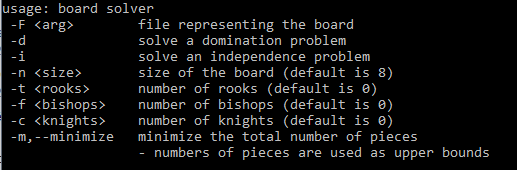
\includegraphics[scale=0.7]{image.png}
\end{center}
On retrouve sur cette images l'ensemble des options disponibles étant donné que le programme réalisé est générique pour les trois problèmes donnés. Les programmes seront lancés via les commandes suivantes : 
\begin{itemize}
\item Domination : -d -n <taille tableau> -c <nombre max> -m
\item Indépendance : -i -n <taille> -c <cavaliers> -t <tours> -f <fous>
\end{itemize}

\subsection{Bonus}
Notre implémentation répond également à la question bonus. Il suffit d'ajouter une fonction reprenant la façon dont la pièce en menace une autre afin de pouvoir l'ajoutée à notre programme.

\section{Surveillance de musée}
La résolution du problème de musée a été réalisée en dérivant les résultats obtenus lors des exercices précédents. On s'est donc directement inspirés du problème de domination afin trouver une réponse adéquate. Avant de commencer le détail du problème sous la forme CSP, détaillons les données fournies avec le problème : 
\begin{equation*}
O = \{(i_{o1},j_{o1}),\ldots,(i_{ok},j_{ok}) \} \vspace{0.1cm} 
\end{equation*}
\begin{equation*}
V = \{ (i_{v1},j_{v1}),\ldots,(i_{vm},j_{vm}) \}
\end{equation*}
Où l'ensemble O représente les positions des cases occupées et l'ensemble V des cases vides. Notons également que la taille en $X$ et en $Y$ sera également fournie avec le problème (les variables du problème seront dénommées par ces deux lettres).
\subsection{Variables}
Les variables qui seront utilisées pour la suite de l'exercice seront définies ici. On retrouvera les caméras est, ouest, nord et sud mais également les cases vides et occupées. Voici les ensembles et variables utilisés : 
\begin{align*}
E =& \ \{ e_1,.., e_n \} \\
W =& \  \{ w_1,.., w_p \} \\
N =& \  \{ n_1,.., n_q \} \\
S =& \  \{ s_1,.., s_r \} \\
T =& \ E \cup W \cup N \cup S
\end{align*}
\begin{equation*}
X = \{x_v \in V \} \cup \{x_e | e \in E \} \cup \{x_w | w \in W\} \cup \{x_n | n \in N\} \cup \{x_s | s \in S \} \cup \{x_o \in O\} 
\end{equation*}
\subsection{Domaines}
Les domaines sont fortement comparables à ceux utilisés dans les exercices précédents : 
\begin{align*}
D_e =& \{ (i,j) \in V \} \\ 
D_w =& \{ (i,j) \in V \} \\ 
D_n =& \{ (i,j) \in V \} \\ 
D_s =& \{ (i,j) \in V \} \\ 
\end{align*}
\subsection{Contraintes}
Les contraintes appliquées sur ce problème seront encore une fois découpées en multiples parties à savoir : 
\begin{center}
\textit{Il n'existe pas de case vide qui soit non occupée et non visée} \vspace{0.1cm} \\
%\textit{Il n'existe pas d'ensembles $| W_1 | + | N_1 | + | S_1 | + | E_1 | \leq  | W | + | N | + | S | + | E |$ qui respecte les deux conditions précédentes et soient différents de $W$, $N$, $S$,  $E$} \vspace{0.1cm} \\
\textit{Il n'existe pas de case ayant deux pièces sur la même case}
\end{center}
On va alors commencer par déterminer qu'il n'existe pas deux pièces au même endroit : 
\begin{equation*}
C_p = \{ C_{p_lp_m} | \ p_l \in T, p_m \in T \backslash \{ p_l \} \}
\end{equation*}
\begin{equation*}
C_{p_lp_m} = ((x_{p_l},x_{p_m}), \{ (i_{p_l},i_{p_m},j_{p_l},j_{p_m}) \in V^2 | \neg((i_{p_l} = i_{p_m}) \wedge (j_{p_l} = j_{p_m}))  \}  )
\end{equation*}
A ce premier ensemble de contraintes, on vient alors ajouter que toutes les cases doivent être occupées ce qui donne : 
\begin{align*}
C_c = \ & \{ C_{e_1c_2} | c_1 \in E, c_2 \in  V \} \ \cup \\
 & \{ C_{w_1c_2} | w_1 \in W, c_2 \in V \} \ \cup \\
 & \{ C_{n_1c_2} | n_1 \in N, c_2 \in V \} \ \cup \\
 & \{ C_{s_1c_2} | s_1 \in S, c_2 \in V \} 
\end{align*}
Ce qui nous donne alors pour chacune des contraintes les résultats suivants : 
\begin{align*}
C_{e_1c_2} = & \ ( (i_{e_1},i_{c_1},j_{e_1},j_{c_1}) \in V^2 | [ j_{e_1} = j_{c_1} ] ) \wedge [i_{e_1} \leq i_{c_1}] \wedge [\nexists x_o | (j_{e_1} = j_o) \wedge (i_{e_1} \leq i_{o} \leq i_{c_1})] \\
C_{w_1c_2} = & \ ( (i_{w_1},i_{c_1},j_{w_1},j_{c_1}) \in V^2 | [ j_{w_1} = j_{c_1} ] ) \wedge [i_{c_1} \leq i_{w_1}] \wedge [\nexists x_o | (j_{w_1} = j_o) \wedge (i_{c_1} \leq i_{o} \leq i_{w_1})] \\
C_{s_1c_2} = & \ ( (i_{s_1},i_{c_1},j_{s_1},j_{c_1}) \in V^2 | [ i_{s_1} = i_{c_1} ] ) \wedge [j_{s_1} \leq j_{c_1}] \wedge [\nexists x_o | (i_{s_1} = i_o) \wedge (j_{s_1} \leq j_{o} \leq j_{c_1})] \\
C_{n_1c_2} = & \ ( (i_{n_1},i_{c_1},j_{n_1},j_{c_1}) \in V^2 | [ i_{n_1} = i_{c_1} ] ) \wedge [j_{c_1} \leq j_{n_1}] \wedge [\nexists x_o | (i_{n_1} = i_o) \wedge (j_{c_1} \leq j_{o} \leq j_{n_1})] 
\end{align*}
Ces quatres contraintes nous assurent donc que pour chaque cases il existe au moins un capteur la visant. Etant donné que nous sommes dans un problème à minimum, il va falloir minimiser l'ensemble des solutions. Pour ce faire, il faut ajouter : 
\begin{align*}
C_s = \{ \nexists \ T_1 | \ (| T_1 | <  | T | ) \wedge (T \neq T_1) \}
\end{align*}
Où $T$ et $T_1$ sont des ensembles formés de $E$,$W$,$N$,$S$. On obtient alors au final : 
\begin{equation*}
C = C_p \cup C_c \cup C_s
\end{equation*}
L'ensemble du code correspondant sera également trouvable en annexe de ce document.
\end{document}








